\documentclass[20pt]{extarticle}
\usepackage[dvips]{graphicx}

\usepackage{mathtools}

\usepackage{geometry}
	\geometry{
	left=3mm,
	right=3mm,
	top=3mm,
	bottom=9mm,
	includefoot,
	footskip=5mm
	}

\usepackage{amssymb,amsmath}

\renewcommand{\labelitemii}{$\blacktriangleright$}

\usepackage{bm}
\usepackage{color}

\usepackage{esvect}

\usepackage{supertabular}
\usepackage{multirow}
\usepackage{bigstrut}

\usepackage{ulem}
\newcommand{\del}[1]{\textcolor{red}{\sout{#1}}}
\newcommand{\ms}[1]{\textcolor{orange}{\bf [Michiko: #1]}}
\newcommand{\add}[1]{\textcolor{blue}{#1}}
\newcommand{\addd}[1]{\textcolor{orange}{#1}}
\newcommand{\naoki}[1]{\textcolor{green}{\bf [Naoki: #1]}}
\newcommand{\tw}[1]{\textcolor{cyan}{\bf [Takamitsu: #1]}}
\newcommand{\tocc}[1]{[\textcolor{cyan}{#1}]}

\usepackage[hidelinks]{hyperref}
\newcommand{\hrefc}[2]{\href{#1}{\textcolor{blue}{#2}}}

\newcommand{\topdir}{../../..}

\usepackage{fancyhdr}
\pagestyle{fancy}
\fancyhf{}
\renewcommand{\headrulewidth}{0pt}
\renewcommand{\footrulewidth}{0pt}
\fancyfoot[R]{\footnotesize\thepage}
\fancypagestyle{plain}{%
	\fancyhf{}%
	\renewcommand{\headrulewidth}{0pt}%
	\renewcommand{\footrulewidth}{0pt}%
	\fancyfoot[R]{\footnotesize\thepage}%
}

\sloppy

\begin{document}

\title{MATH 463 Mathematical Biology\\ lecture notes\\
10. Mathematical ecology}
\date{\today}
\author{Naoki Masuda}

\maketitle

\begin{itemize}
\item Mathematical ecology models how populations and communities of organisms change over time and space. Classic topics include:
	\begin{itemize}
	\item single-species growth (exponential, logistic),
	\item predator--prey and competition models (Lotka--Volterra).
	\end{itemize}
\item Here we focus on a few more advanced themes:
	\begin{itemize}
	\item \textbf{Coexistence}: why do so many species coexist in an ecosystem? This is non-trivial.
	\item \textbf{Tipping points}: can we anticipate sudden, catastrophic ecological shifts \emph{before} they happen?
	\end{itemize}
\end{itemize}

\subsection*{Why do many species coexist?}

\begin{itemize}
\item A long-standing intuition in ecology (\hrefc{https://doi.org/10.2307/1929601}{MacArthur, Ecology (1955)}; \hrefc{https://doi.org/10.1007/978-1-4899-7214-9}{Elton's book (1958)}) was that more complex (i.e., more species, more interactions) communities are more stable, e.g.\ more resistant to invasions or to the loss of a species.
	\begin{itemize}
	\item MacArthur's claim is based on linear dynamics \& entropy arguments.
	\end{itemize}
\item In 1972, Robert May challenged this intuition with a simple mathematical argument (\hrefc{https://doi.org/10.1038/238413a0}{May, Nature (1972)}).
\end{itemize}

\subsubsection*{May's random community matrix}

\begin{itemize}
\item Consider a community of $S$ species at an equilibrium $\vec{x}^* = \begin{pmatrix} x_1^* \\ \vdots \\ x_S^* \end{pmatrix}$. 
\item Linearize the (unspecified) population dynamics around that equilibrium:
\[ \frac{\text{d}\vec{x}}{\text{d}t} = f(\vec{x}),\quad \vec{x} = \begin{pmatrix} x_1 \\ \vdots \\ x_S \end{pmatrix}, \]
where $f$ is an unspecified function modeling population dynamics.\\
A small deviation from the equilibrium: $\vec{z} = \vec{x} - \vec{x}^*$.
	\begin{itemize}
	\item \textbf{Q:} Why a \emph{small} deviation?
	\item \textbf{Q:} Taylor expand $f(\vec{x})$ around $\vec{x} = \vec{x}^*$.
	\end{itemize}
The local dynamics of the small deviations $\vec{x}$ are
\[ \frac{\text{d}\vec{x}}{\text{d}t} = M \vec{x}, \]
where $M$ is the $S\times S$ \emph{community matrix} (the Jacobian).\\
$M_{ij}$ is the effect of species $j$ on the growth of species $i$ near equilibrium.
\item The equilibrium is (locally) stable iff every eigenvalue of $M$ has negative real part.
\item Consider a random matrix $M$:
	\begin{itemize}
	\item Set $M_{ii} = -1$ (each species is self-regulating);
	\item Each off-diagonal pair of species interacts with probability $C$ (the \emph{connectance}).
	\item A present interaction $M_{ij}$ (occurring with probability $C$) is drawn from a distribution with mean $0$ and variance $\sigma^2$.
	\item Absent interactions are $0$.
	\end{itemize}
\item For large $S$, the eigenvalues of $M$ fill a disk in the complex plane centered at $(-1,0)$ with radius $\sigma\sqrt{SC}$.
	\begin{itemize}
	\item \textbf{Exercise:} Draw it in the complex plane.
	\end{itemize}
	The dynamical system is almost surely stable iff
\vspace{6cm}
\[ \sigma\sqrt{SC} < 1. \]
\item Paradox: Increasing the ``complexity''
	\begin{itemize}
	\item more species $S$,
	\item denser connectance $C$, or
	\item stronger interactions $\sigma$
	\end{itemize}
	\emph{destabilizes} the community. This is the opposite of the older intuition. So,
	\begin{quote}
	If random complex communities are almost surely unstable, how do real, species-rich ecosystems persist?
	\end{quote}
\item This launched the ``diversity--stability debate.'' Some proposed mechanisms supporting stability are:
\end{itemize}

\subsubsection*{Mechanism 1: many weak interactions}

\begin{itemize}
\item \hrefc{https://doi.org/10.1038/27427}{McCann, Hastings \& Huxel, Nature (1998)} showed that a preponderance of \emph{weak} interactions (rather than a few strong ones) dampens population oscillations and stabilizes food webs. 
\item Weak links act as a buffer, keeping consumer--resource cycles from blowing up.
\item Real food webs are indeed dominated by many weak interactions.
\end{itemize}

\subsubsection*{Mechanism 2: interaction types and food-web structure}

\begin{itemize}
\item \hrefc{https://doi.org/10.1038/nature10832}{Allesina \& Tang, Nature (2012)} extended May's random-matrix analysis to realistic pairwise interaction types, where the signs of $M_{ij}$ and $M_{ji}$ are constrained:
	\begin{itemize}
	\item \emph{predator--prey} ($+/-$): if $M_{ij}>0$ then $M_{ji}<0$,
	\item \emph{mutualism} ($+/+$),
	\item \emph{competition} ($-/-$).
	\end{itemize}
\item The shape of the eigenvalue cloud changes with the interaction type:
\begin{center}
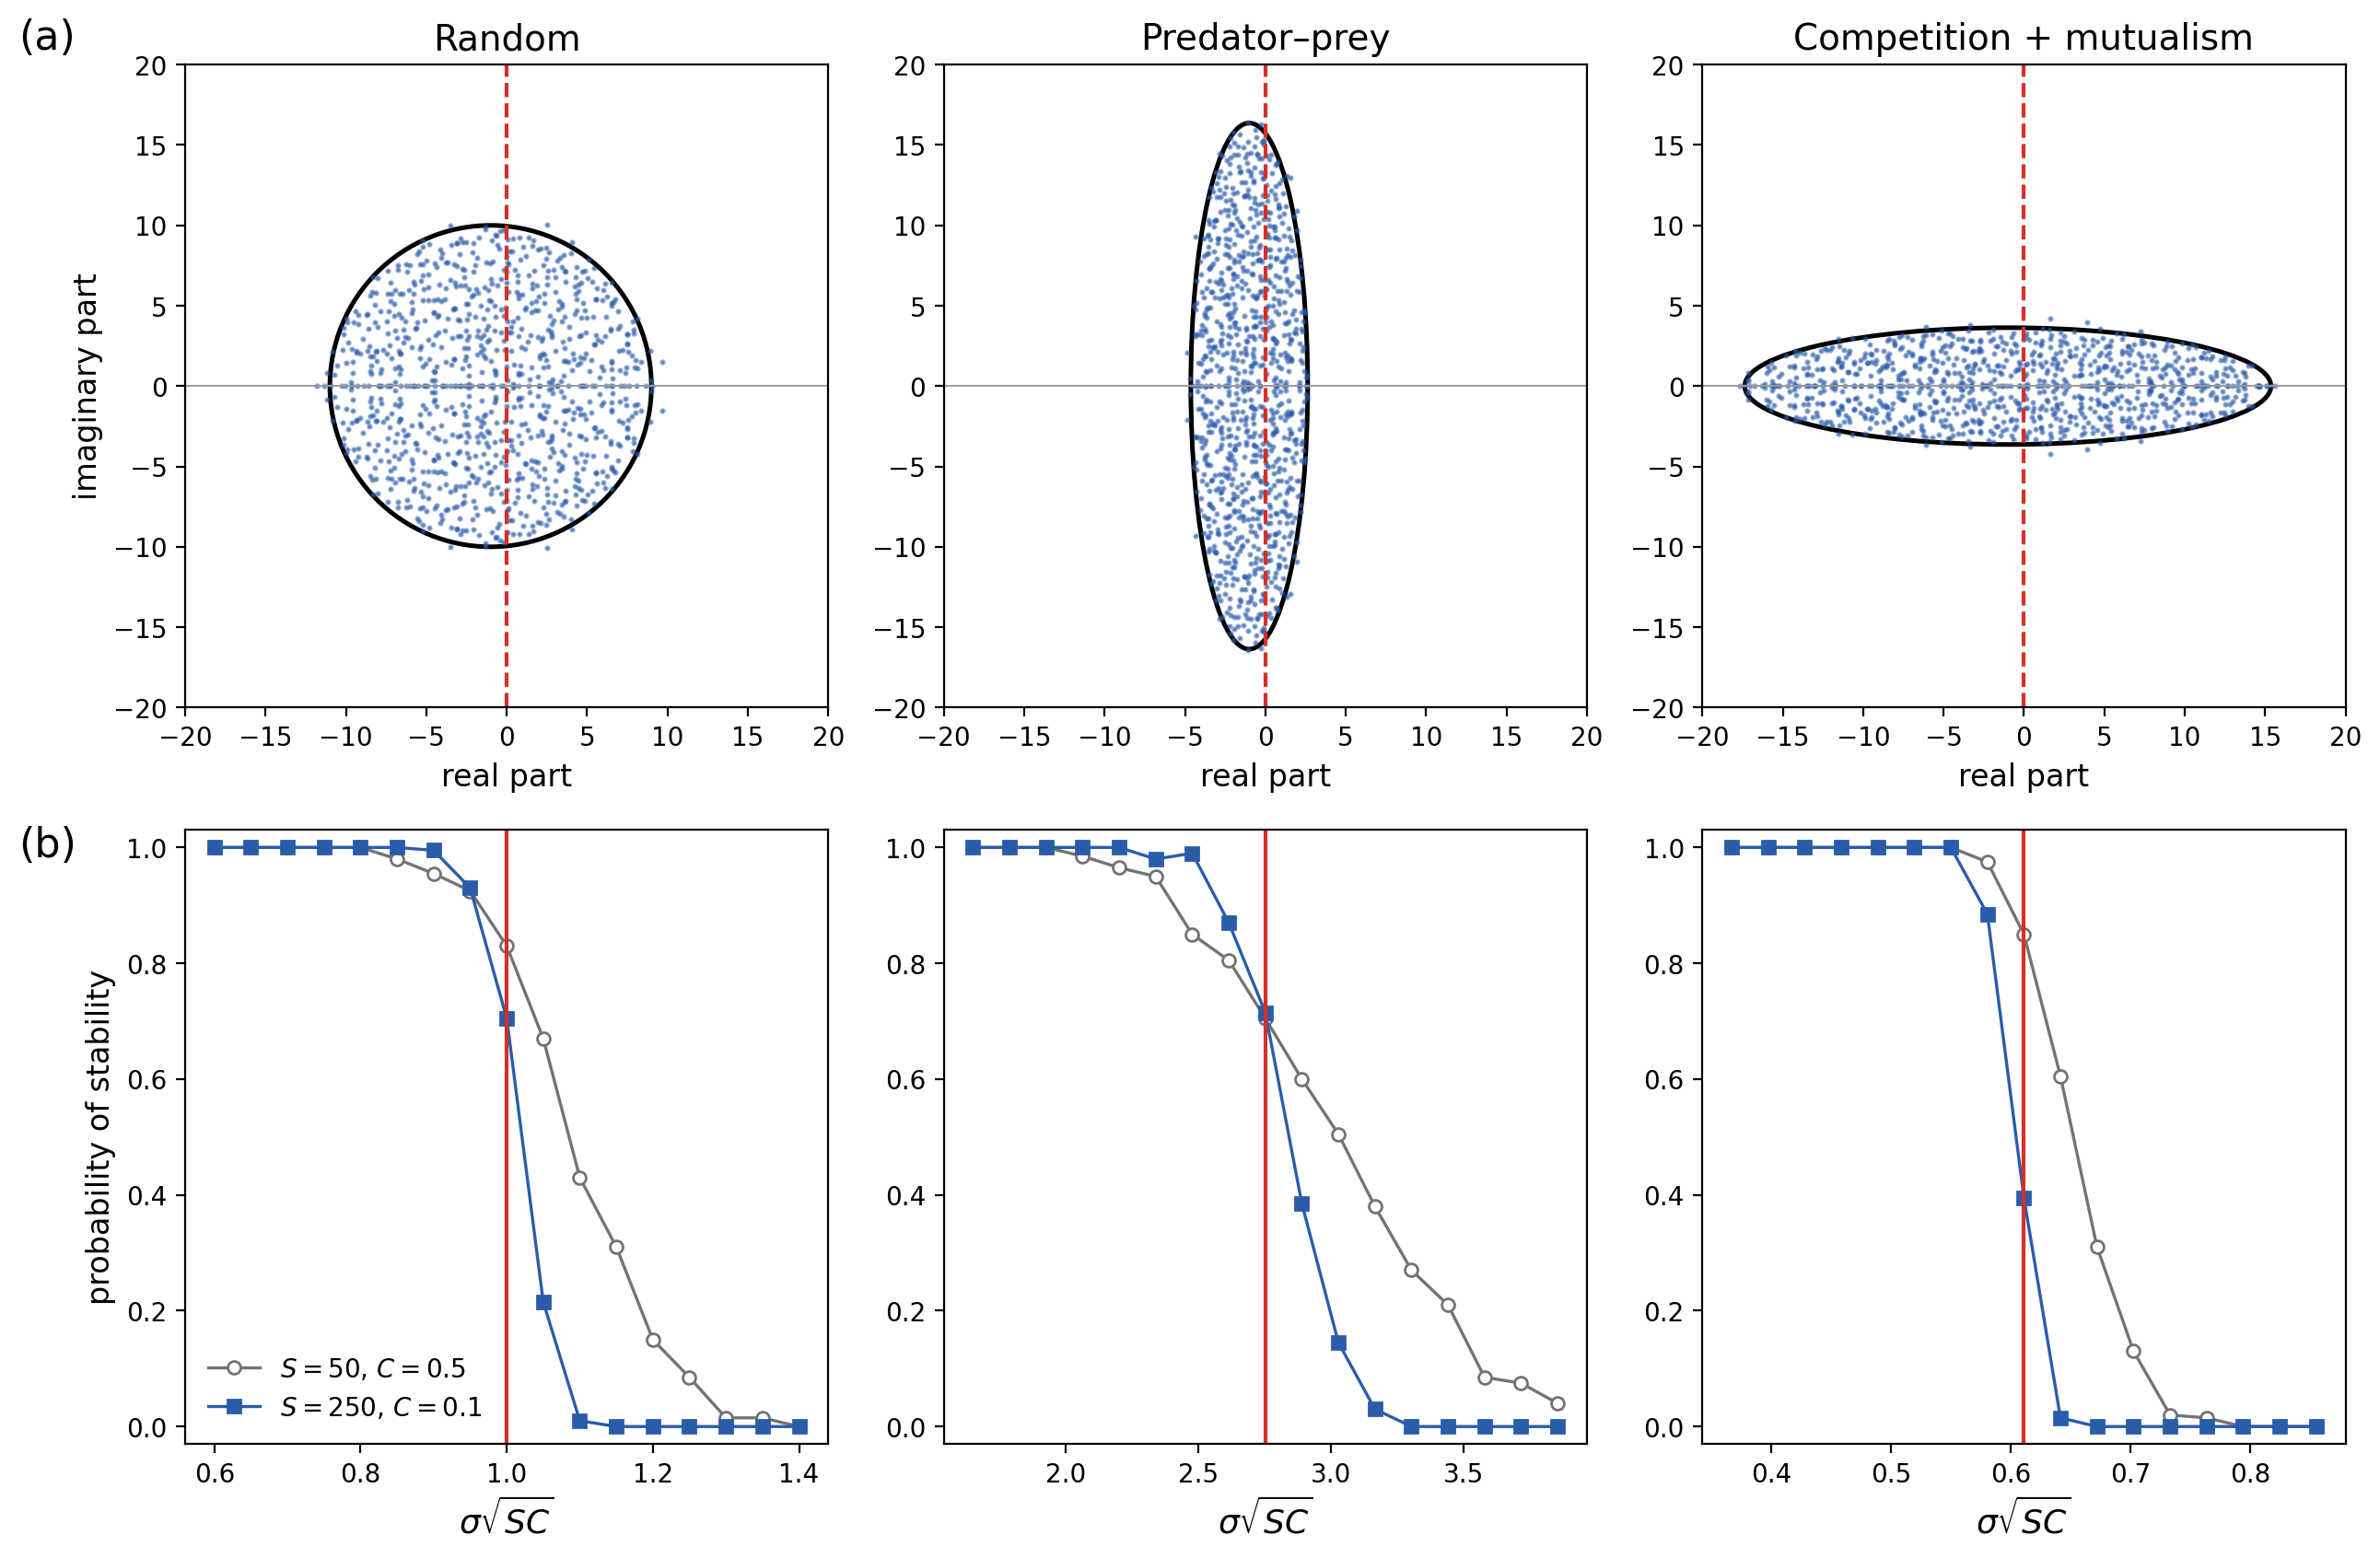
\includegraphics[width=\linewidth]{figures/10_mathematical_ecology/random-community-stability.png}\\
\end{center}
Figure: (a) Eigenvalues of the community matrix for three types of interactions ($S=250$, $C=0.25$, diagonal $-1$); the black curves are the theoretical circle and ellipses. Red dashed line: stability boundary. (b) Probability of stability; the red lines are the analytical thresholds. Own simulation, after Fig.~1 of \hrefc{https://doi.org/10.1038/nature10832}{Allesina \& Tang, Nature (2012)}.
	\begin{itemize}
	\item \textbf{Q:} Which one is the best?
	\ \\
	\ \\
	\ \\
	\item random: a disk (May's case);
	\item predator--prey: a vertically stretched ellipse --- narrower in the real direction, so it is stabilizing;
	\item mutualism/competition: a horizontally stretched ellipse --- wider in the real direction, so it is destabilizing.
	\end{itemize}
\item Lessons:
	\begin{itemize} 
	\item Predator--prey-dominated food webs can be much larger and more complex while remaining stable than May's random communities.
	\item Mutualistic/competitive webs are more fragile.
	\item Structure and interaction type, not just raw complexity, govern stability.
	\end{itemize}
\end{itemize}

\subsubsection*{Mechanism 3: adaptive foraging}

\begin{itemize}
\item \hrefc{https://doi.org/10.1126/science.1079154}{Kondoh, Science (2003)} proposed \emph{adaptive foraging}: consumers continually re-allocate their foraging effort toward whichever prey is currently most profitable (``prey switching''). 
\item The who-eats-whom network is therefore dynamic (temporal, or time-varying, networks).
\item Model: the biomass $X_i$ of species $i$ ($i = 1,\ldots,N$) obeys a Lotka--Volterra-type system
\[
\begin{aligned}
\frac{\text{d}X_i}{\text{d}t} = X_i\Bigg( r_i - s_i X_i
&+ \sum_{j\,\in\,\text{resources}} e\, f_{ij} a_{ij} X_j\\
&- \sum_{j\,\in\,\text{consumers}} f_{ji} a_{ji} X_j \Bigg),
\end{aligned}
\]
where
	\begin{itemize}
	\item $r_i =$ intrinsic growth rate,
	\item $s_i =$ self-regulation,
	\item $f_{ij} =$ foraging efficiency of $i$ on resource $j$, and
	\item $e =$ conversion efficiency.
	\end{itemize}
\item The key new ingredient is the \emph{foraging effort} $a_{ij}$ that species $i$ allocates to resource $j$, with the budget constraint
\[ \sum_{j} a_{ij} = 1. \]
$a_{ij}$ changes over time, with a consumer shifting more of its effort toward whichever resource currently yields the higher per-capita intake rate (i.e., the more abundant or more easily caught prey).\\
This is \emph{adaptive foraging} (prey switching).
\item \textbf{Result:} 
	\begin{itemize}
	\item Without adaptive foragers, complexity destabilizes (as in May).
	\item With adaptive foraging, complexity can \emph{enhance} community persistence --- the complexity--stability relationship can turn positive.
		\begin{itemize}
		\item Intuition: Prey switching reroutes energy away from over-exploited species.
		\end{itemize}
	\end{itemize}
\end{itemize}

\subsection*{Rock--paper--scissors dynamics and the maintenance of diversity}

\begin{itemize}
\item Another route to coexistence of species is \emph{non-transitive} competition.\\
A cyclic ``rock beats scissors beats paper beats rock'' relationship has no overall winner, so diversity can persist with cyclic dynamics.
\end{itemize}

\subsubsection*{Experiment 1: lizards}

\begin{itemize}
\item In the lizard \textit{Uta stansburiana}, males come in three throat-color morphs, each a different mating strategy (\hrefc{https://doi.org/10.1038/380240a0}{Sinervo and Lively, Nature (1996)}):
	\begin{itemize}
	\item \textbf{orange}: very aggressive, defends a large territory with many females;
	\item \textbf{blue}: less aggressive, guards a single female;
	\item \textbf{yellow}: ``sneaker,'' mimics females and sneaks copulations.
	\end{itemize}
\item These beat each other cyclically.
	\begin{itemize}
	\item Orange (large territories) overpowers blue.
	\item Blue (mate-guarding) thwarts yellow sneakers.
	\item Yellow sneakers exploit orange males who cannot watch all their females.
	\end{itemize}
\item Selection is frequency-dependent: each morph does best when rare. As a result, the morph frequencies oscillate over the years.
\end{itemize}

\begin{figure}[h]
\begin{center}
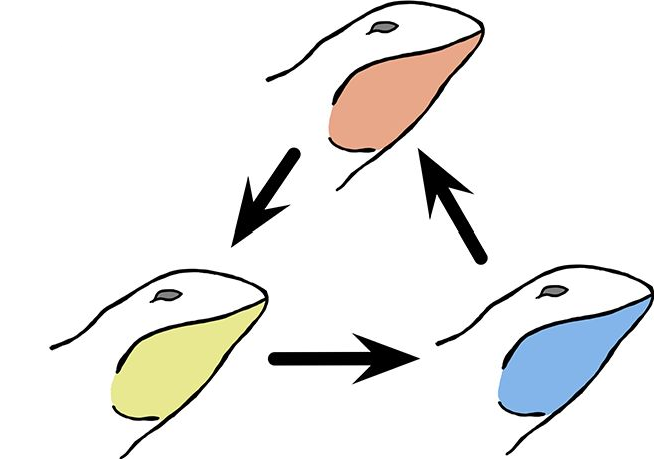
\includegraphics[width=0.4\textwidth]{figures/10_mathematical_ecology/Park2020-lizards.png}\\[3mm]
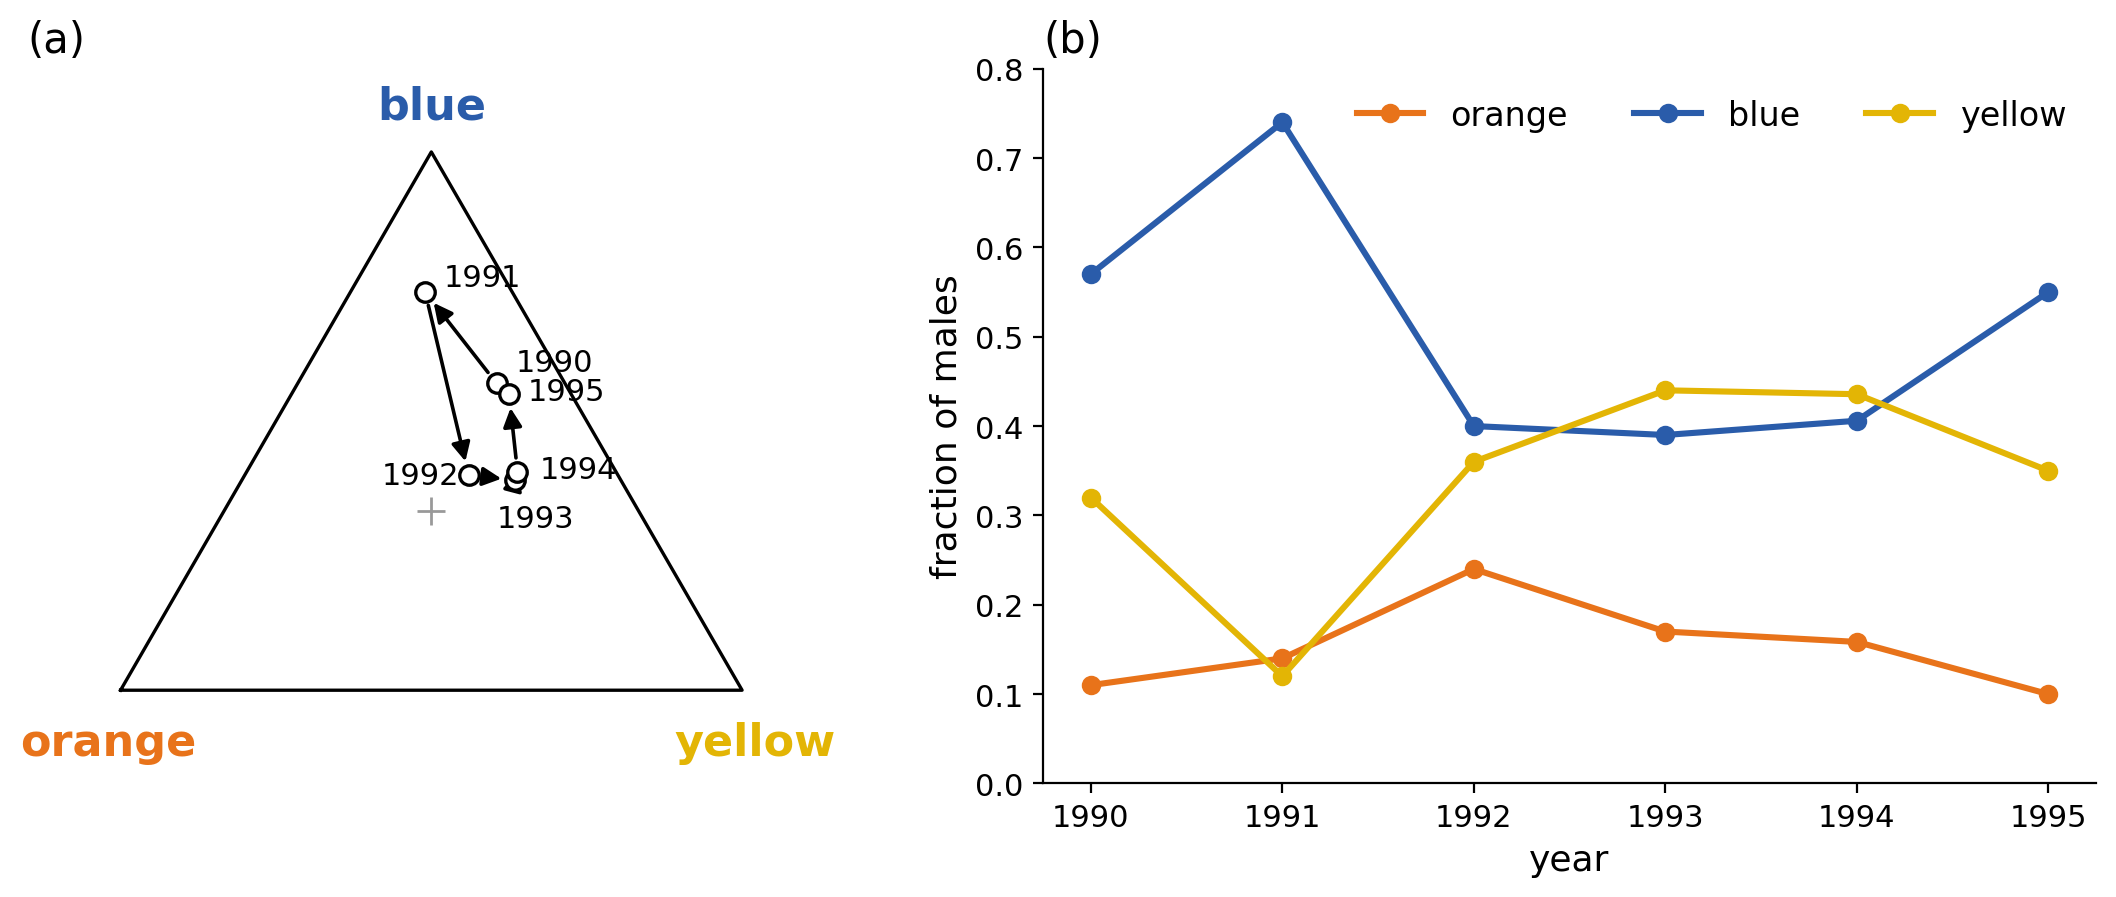
\includegraphics[width=\textwidth]{figures/10_mathematical_ecology/lizard-morph-cycle.png}
\caption{Top: the three throat-color morphs of male side-blotched lizards \textit{Uta stansburiana}. An arrow points from the dominated morph to the dominant one. Figure~1C of \hrefc{https://doi.org/10.7554/eLife.57857}{Park, Pichugin \& Traulsen, eLife (2020)}, licensed under \hrefc{https://creativecommons.org/licenses/by/4.0/}{CC BY 4.0}. Bottom: frequencies of the three morphs among males from 1990 to 1995, (a) on the simplex and (b) over time. Redrawn from data read off Fig.~2 of \hrefc{https://doi.org/10.1038/380240a0}{Sinervo \& Lively, Nature (1996)}.}
\label{fig:lizard}
\end{center}
\end{figure}

\clearpage

\subsubsection*{Experiment 2: \textit{E.\ coli} colicin system}

\begin{itemize}
\item \hrefc{https://doi.org/10.1038/nature00823}{Kerr, Riley, Feldman and Bohannan, Nature (2002)} built a microbial rock--paper--scissors with three strains of \textit{Escherichia coli}:
	\begin{itemize}
	\item \textbf{C}: colicin \emph{producer} (makes a toxin that kills sensitive cells, at a metabolic cost);
	\item \textbf{S}: colicin \emph{sensitive} (fast grower, but killed by colicin);
	\item \textbf{R}: colicin \emph{resistant} (immune, but pays a resistance cost, so grows slower than S).
	\end{itemize}
\item Cycle:
	\begin{itemize}
	\item C kills S.
	\item S outgrows R (S grows fastest).
	\item R outgrows C (R avoids the cost of producing toxin).
	\end{itemize}
\item Result: space matters:
	\begin{itemize}
	\item On a static plate (local interactions/dispersal), all three strains coexist: local clumps of each type chase each other across the plate.
	\item In a well-mixed flask (global interactions), diversity collapses: C drives S extinct, then R outcompetes C.
	\end{itemize}
\end{itemize}

\begin{figure}[h]
\begin{center}
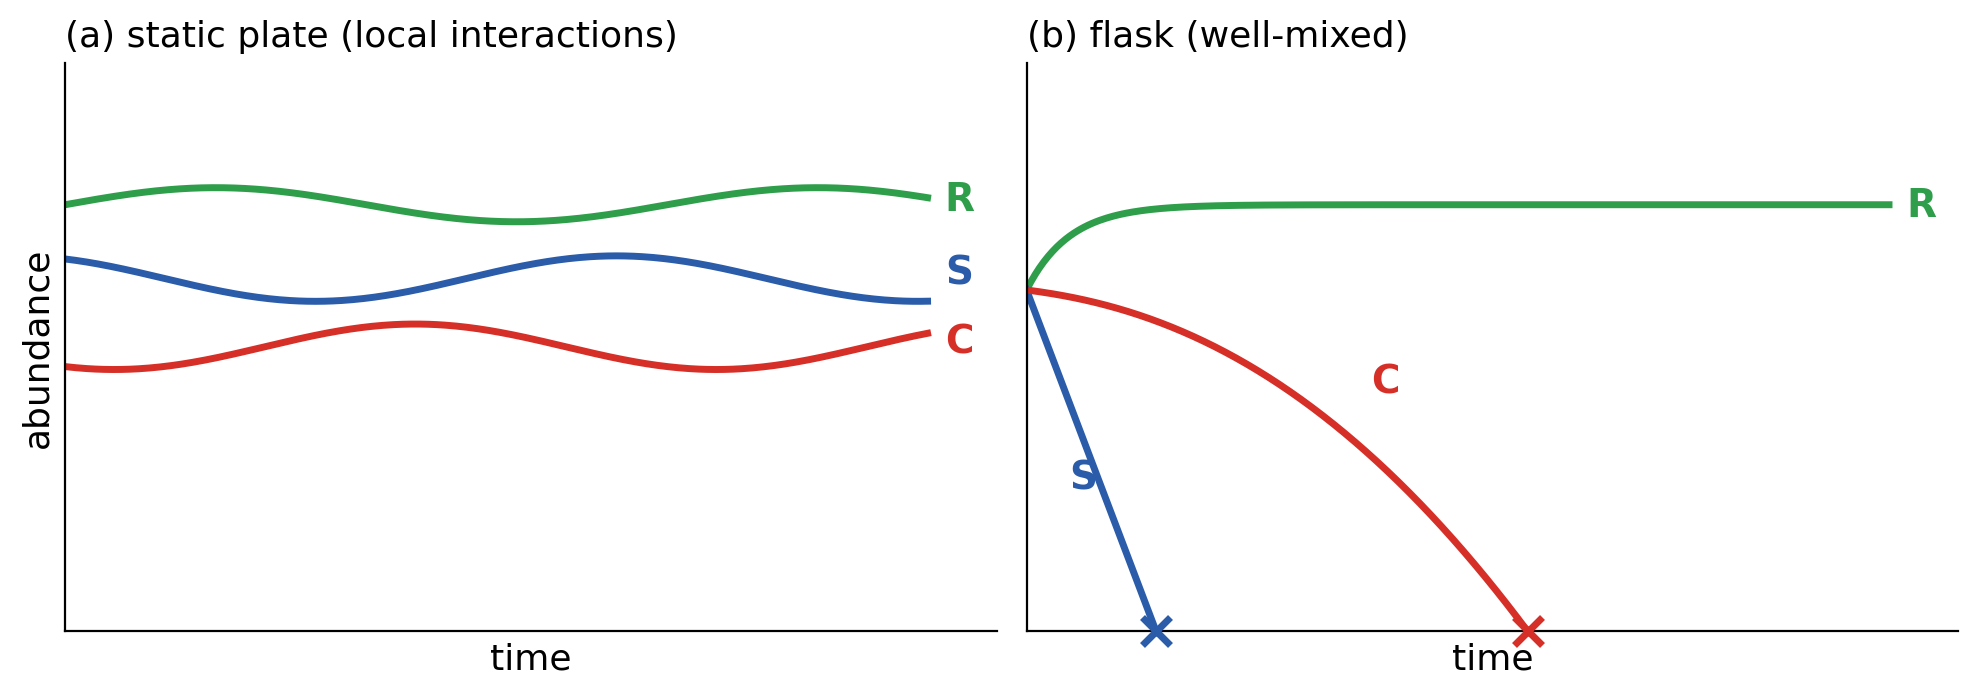
\includegraphics[width=0.85\textwidth]{figures/10_mathematical_ecology/kerr-schematic.png}
\caption{Schematic of dynamics of the C--S--R \textit{E.\ coli} system. (a) Static plate (local interactions). (b) Flask (well-mixed). A schematic summary of the experimental results of \hrefc{https://doi.org/10.1038/nature00823}{Kerr et al., Nature (2002)}; the curves are not meant to be accurate.}
\label{fig:kerr}
\end{center}
\end{figure}

\begin{figure}[h]
\begin{center}
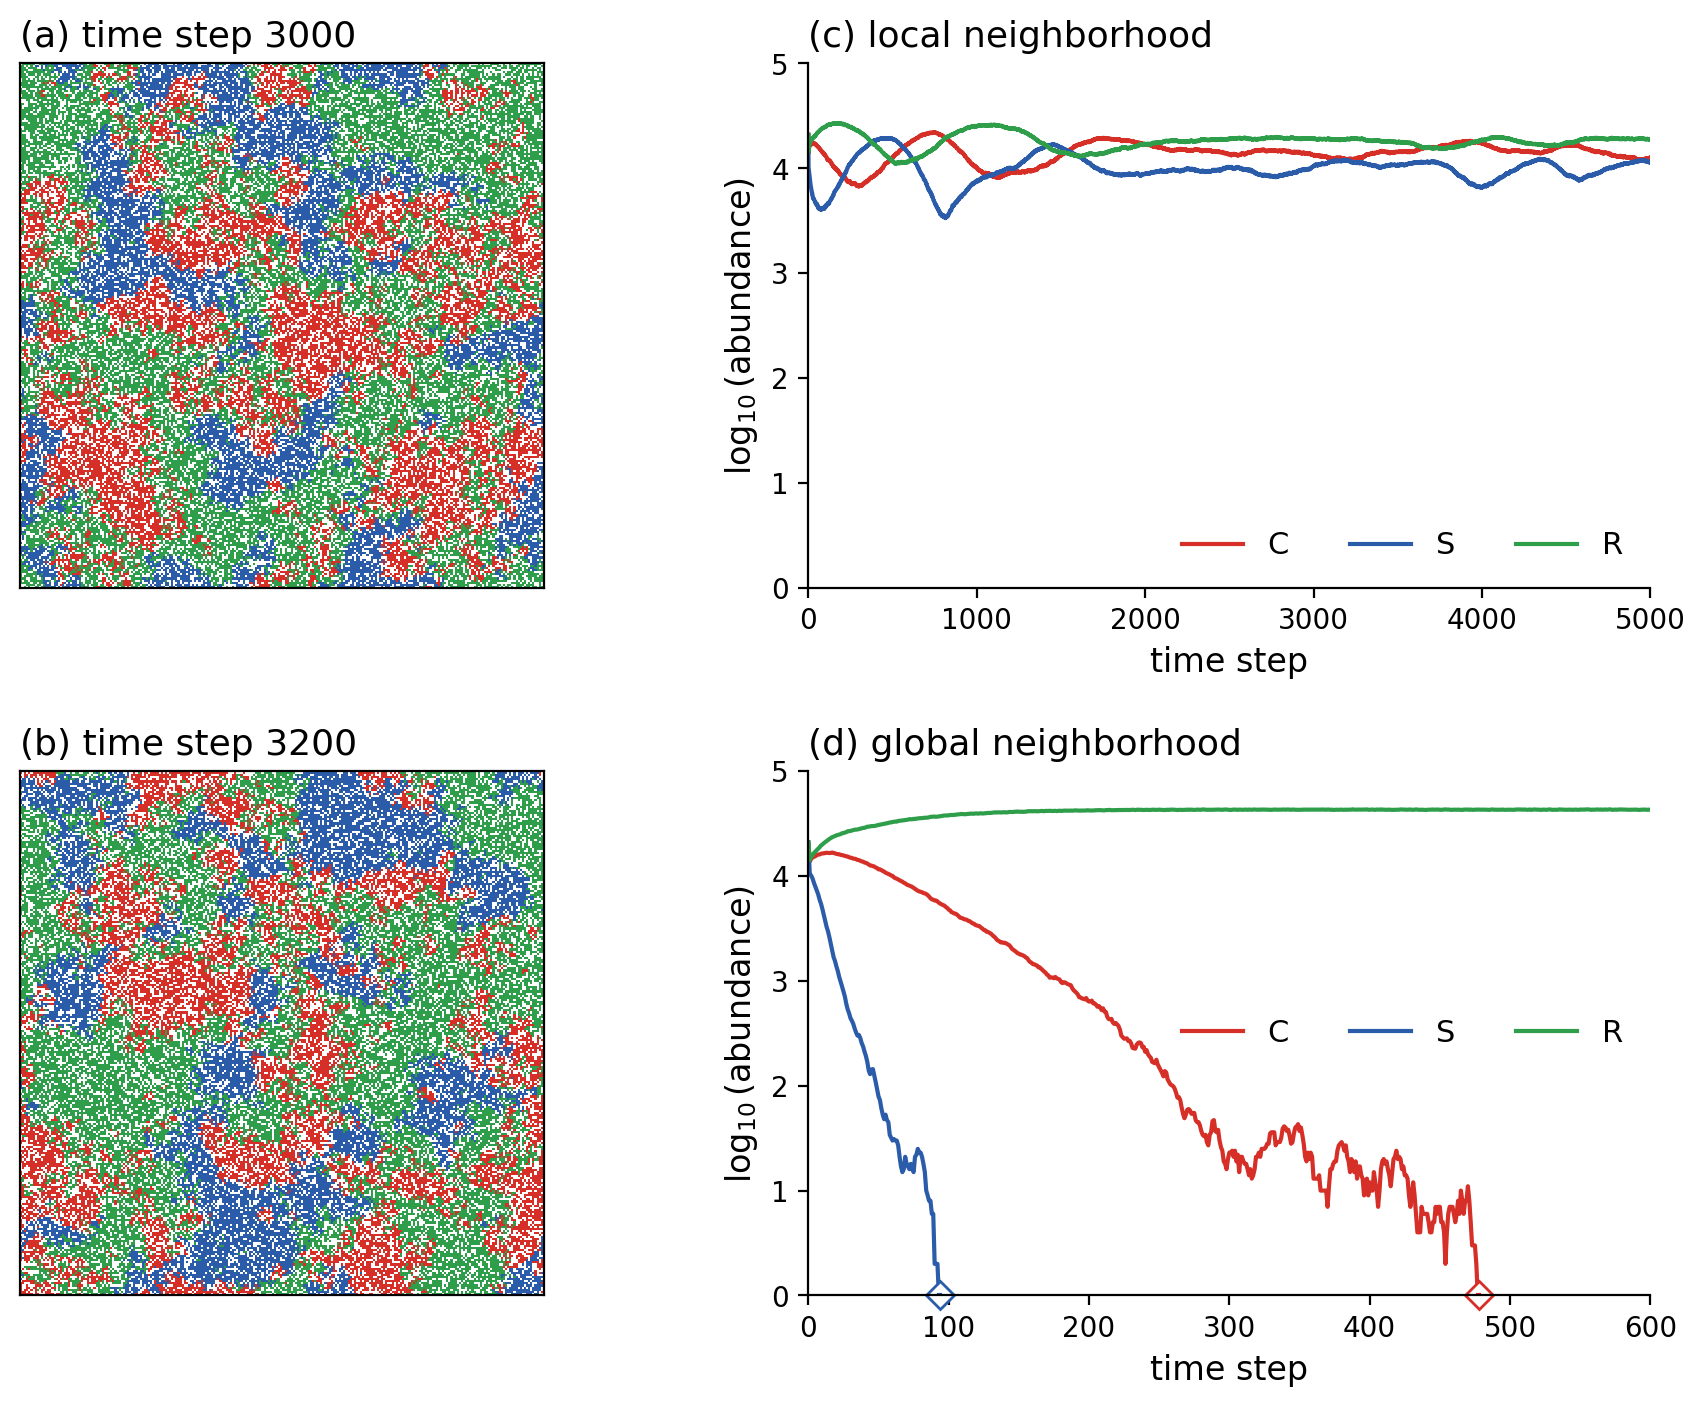
\includegraphics[width=0.85\textwidth]{figures/10_mathematical_ecology/kerr-lattice-sim.png}
\caption{Lattice simulation of the C--S--R system. In the snapshots shown in (a) and (b), local clumps of the three strains chase each other. (c) Local neighborhood (8 nearest sites). (d) Global neighborhood (whole lattice); diamonds mark extinctions. Own simulation, after Fig.~2a--d of \hrefc{https://doi.org/10.1038/nature00823}{Kerr et al., Nature (2002)}.}
\label{fig:kerr-numerical}
\end{center}
\end{figure}

\clearpage

\subsubsection*{A mean-field model: well-mixed interacting particles}

\begin{itemize}
\item Consider a population of individuals, each of one of three types, R, S, P.
\item R beats S, S beats P, and P beats R.
\item When two individuals of different types meet, the dominant one converts the other to its own type:
\[ \text{R} + \text{S} \to \text{R} + \text{R}, \qquad \text{S} + \text{P} \to \text{S} + \text{S}, \qquad \text{P} + \text{R} \to \text{P} + \text{P}. \]
	\begin{itemize}
	\item \textbf{Q:} Similarities and differences from the SIS model?
	\end{itemize}
\item Let $r,s,p$ be the fractions of R, S, P, with $r+s+p=1$.
\item In a well-mixed population, the rate of encounter between two types is proportional to the product of their fractions (\emph{mass action}). $\to$ the
cyclic Lotka--Volterra model:
\item \textbf{Q:} Write down the ODE system.
\ \\
\ \\
\ \\
\ \\
\[
\begin{aligned}
\frac{\text{d}r}{\text{d}t} &= r\,(s - p),\\
\frac{\text{d}s}{\text{d}t} &= s\,(p - r),\\
\frac{\text{d}p}{\text{d}t} &= p\,(r - s).
\end{aligned}
\]
\item \textbf{Exercises:}
	\begin{itemize}
	\item Show $r+s+p=1$ for all $t$. What does this mean?
	\item Get all the equilibria.
	\item Advanced: Show that $H \equiv rsp$ is conserved (i.e., $H$ does not change over time).
		\begin{itemize}
		\item Hence trajectories are closed orbits, and the internal equilibrium is a \emph{neutrally stable center} (Fig.~\ref{fig:rps}). The composition cycles forever. Is this realistic?
		\end{itemize}
	\end{itemize}
\item Take-home: in a well-mixed population, the three types cycle, but the cycles are only \emph{neutrally} stable, so not robust. Any perturbation moves the system onto a different orbit, and in a \emph{finite} population the unavoidable fluctuations make the orbit drift outward until one type, and then a second, goes extinct (Fig.~\ref{fig:rps}, middle). So, coexistence in a well-mixed population is fragile.
\end{itemize}

\begin{figure}[h]
\begin{center}
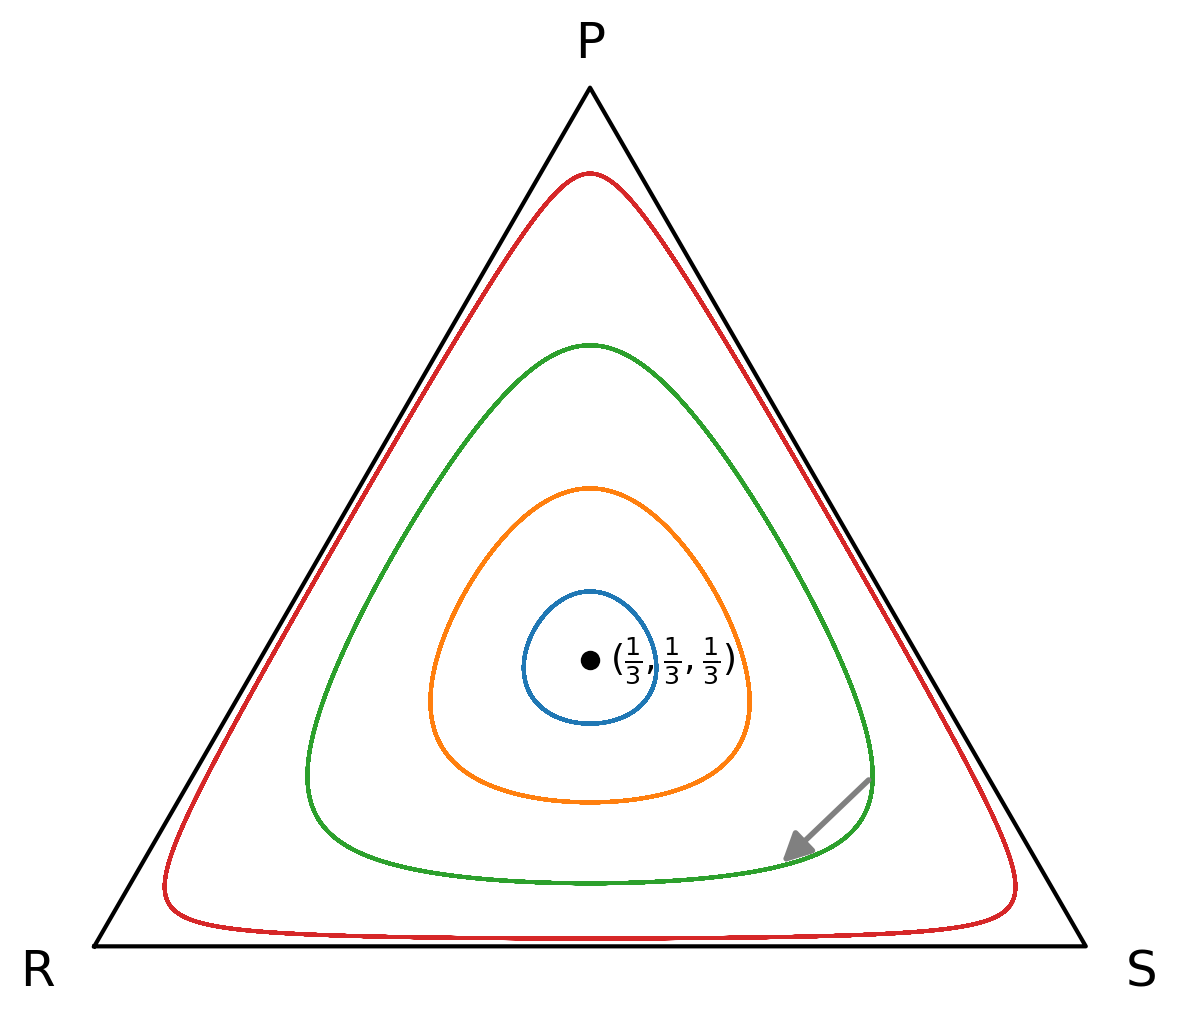
\includegraphics[width=0.32\textwidth]{figures/10_mathematical_ecology/rps-meanfield.png}
\hfill
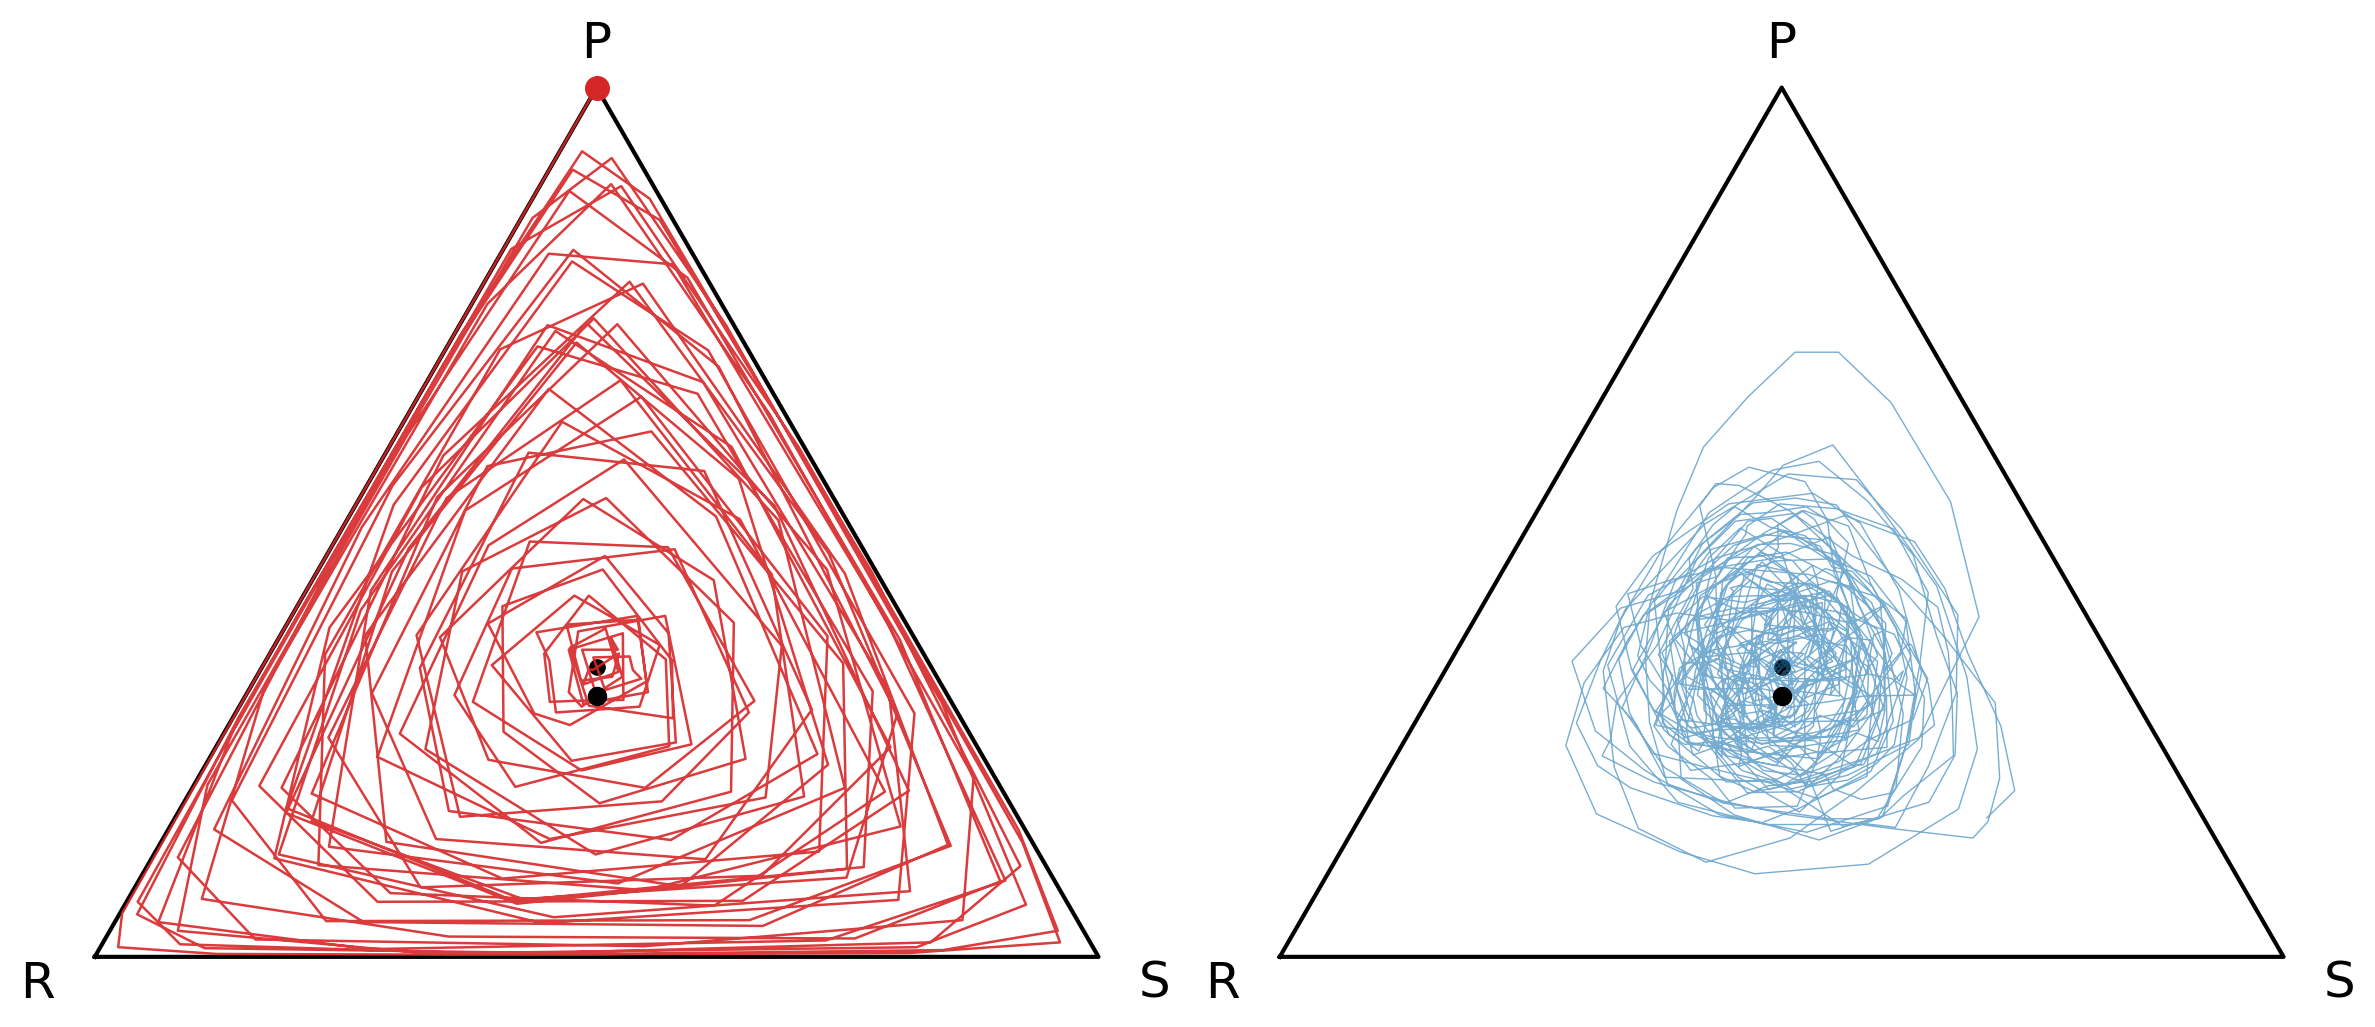
\includegraphics[width=0.64\textwidth]{figures/10_mathematical_ecology/rps-finite-sims.png}
\caption{Rock--paper--scissors dynamics on the \emph{simplex} $r+s+p=1$. In all triangles, the flow occurs clockwise (i.e., $\text{R}\to\text{P}\to\text{S}\to\text{R}$).
Left: the mean-field ($=$ well-mixed) ODE. The interior equilibrium $(\tfrac13,\tfrac13,\tfrac13)$ is a neutrally stable center surrounded by closed orbits.
Middle: well-mixed population of $N=900$ individuals. The orbit winds outward, eventually leaving only P (red dot). \textbf{Q:} Which goes extinct first, R or S?
Right: Square lattice of $N = 30\times30$ individuals. Local interactions keep the composition circulating around $(\tfrac13,\tfrac13,\tfrac13)$ without reaching any corner.}
\label{fig:rps}
\end{center}
\end{figure}

\clearpage

\subsubsection*{Spatial structure}

\begin{itemize}
\item Real populations are not well-mixed: individuals interact \emph{locally}, with their neighbors. Kerr's static-plate experiment already hinted that local interactions can rescue coexistence, and so does the lattice simulation in Fig.~\ref{fig:rps} (right).
\item To study this we place individuals on a lattice and \emph{simulate} (the spatial model is generally not solvable by hand). A (square) lattice means:
\vspace{4cm}
\item \hrefc{https://doi.org/10.1038/nature06095}{Reichenbach, Mobilia \& Frey, Nature (2007)}: Each site of a square lattice is either empty or occupied by an R, S, or P individual. One repeatedly picks a random individual and a random nearest neighbor and applies one of three moves:
\begin{figure}[h]
\begin{center}
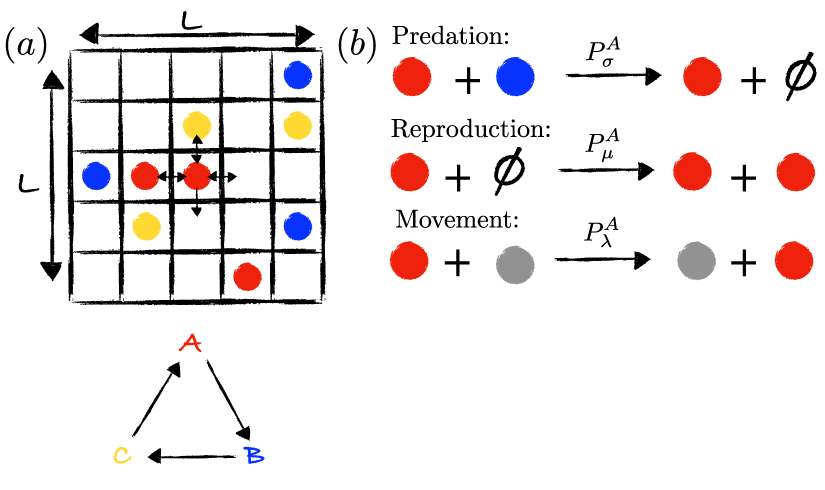
\includegraphics[width=0.7\textwidth]{figures/10_mathematical_ecology/YuJack2025-rules.png}
\caption{Rules of the lattice rock--paper--scissors model with species A (red), B (blue), and C (yellow). (a) Each individual interacts with its four nearest neighbors; A beats B, B beats C, and C beats A. (b) The three moves, shown for species A; $\emptyset$ is an empty site, and gray is any neighbor. The superscripts and subscripts on $P$ label the species and the move; the movement rate $\lambda$ corresponds to $\epsilon$ in the text. Adapted from Fig.~1 of \hrefc{https://doi.org/10.1088/1367-2630/adfd05}{Yu \& Jack, New J.\ Phys.\ (2025)}, licensed under \hrefc{https://creativecommons.org/licenses/by/4.0/}{CC BY 4.0}.}
\label{fig:reich-rules}
\end{center}
\end{figure}
	\begin{itemize}
	\item \textbf{selection (predation)} (rate $\sigma$): if the neighbor is the type that the focal individual dominates, the neighbor is killed and its site becomes empty (e.g.\ R next to S $\Rightarrow$ S is removed);
	\item \textbf{reproduction} (rate $\mu$): if the neighbor site is empty, the focal individual places an offspring of its own type there;
	\item \textbf{exchange (mobility)} (rate $\epsilon$): the focal individual and its neighbor swap places, which lets individuals move around.
	\end{itemize}
\end{itemize}

Results:
\begin{itemize}
\item The three types self-organize into rotating spiral waves.
\item All three types persist, unlike the well-mixed model.
\item Matches the plate (local) vs.\,flask (well-mixed) contrast of Kerr's experiment.
\item Mobility jeopardizes biodiversity. There is a critical mobility $\epsilon_{\rm c}$:
	\begin{itemize}
	\item below $\epsilon_{\rm c}$: small spirals form and all three types coexist indefinitely;
	\item above $\epsilon_{\rm c}$: the spirals grow until their wavelength ($\approx$ spiral size) exceeds the system size, the patterns wash out (the population becomes effectively well-mixed), and two of the three types go extinct.
	\end{itemize}
\end{itemize}

\begin{figure}[h]
\begin{center}
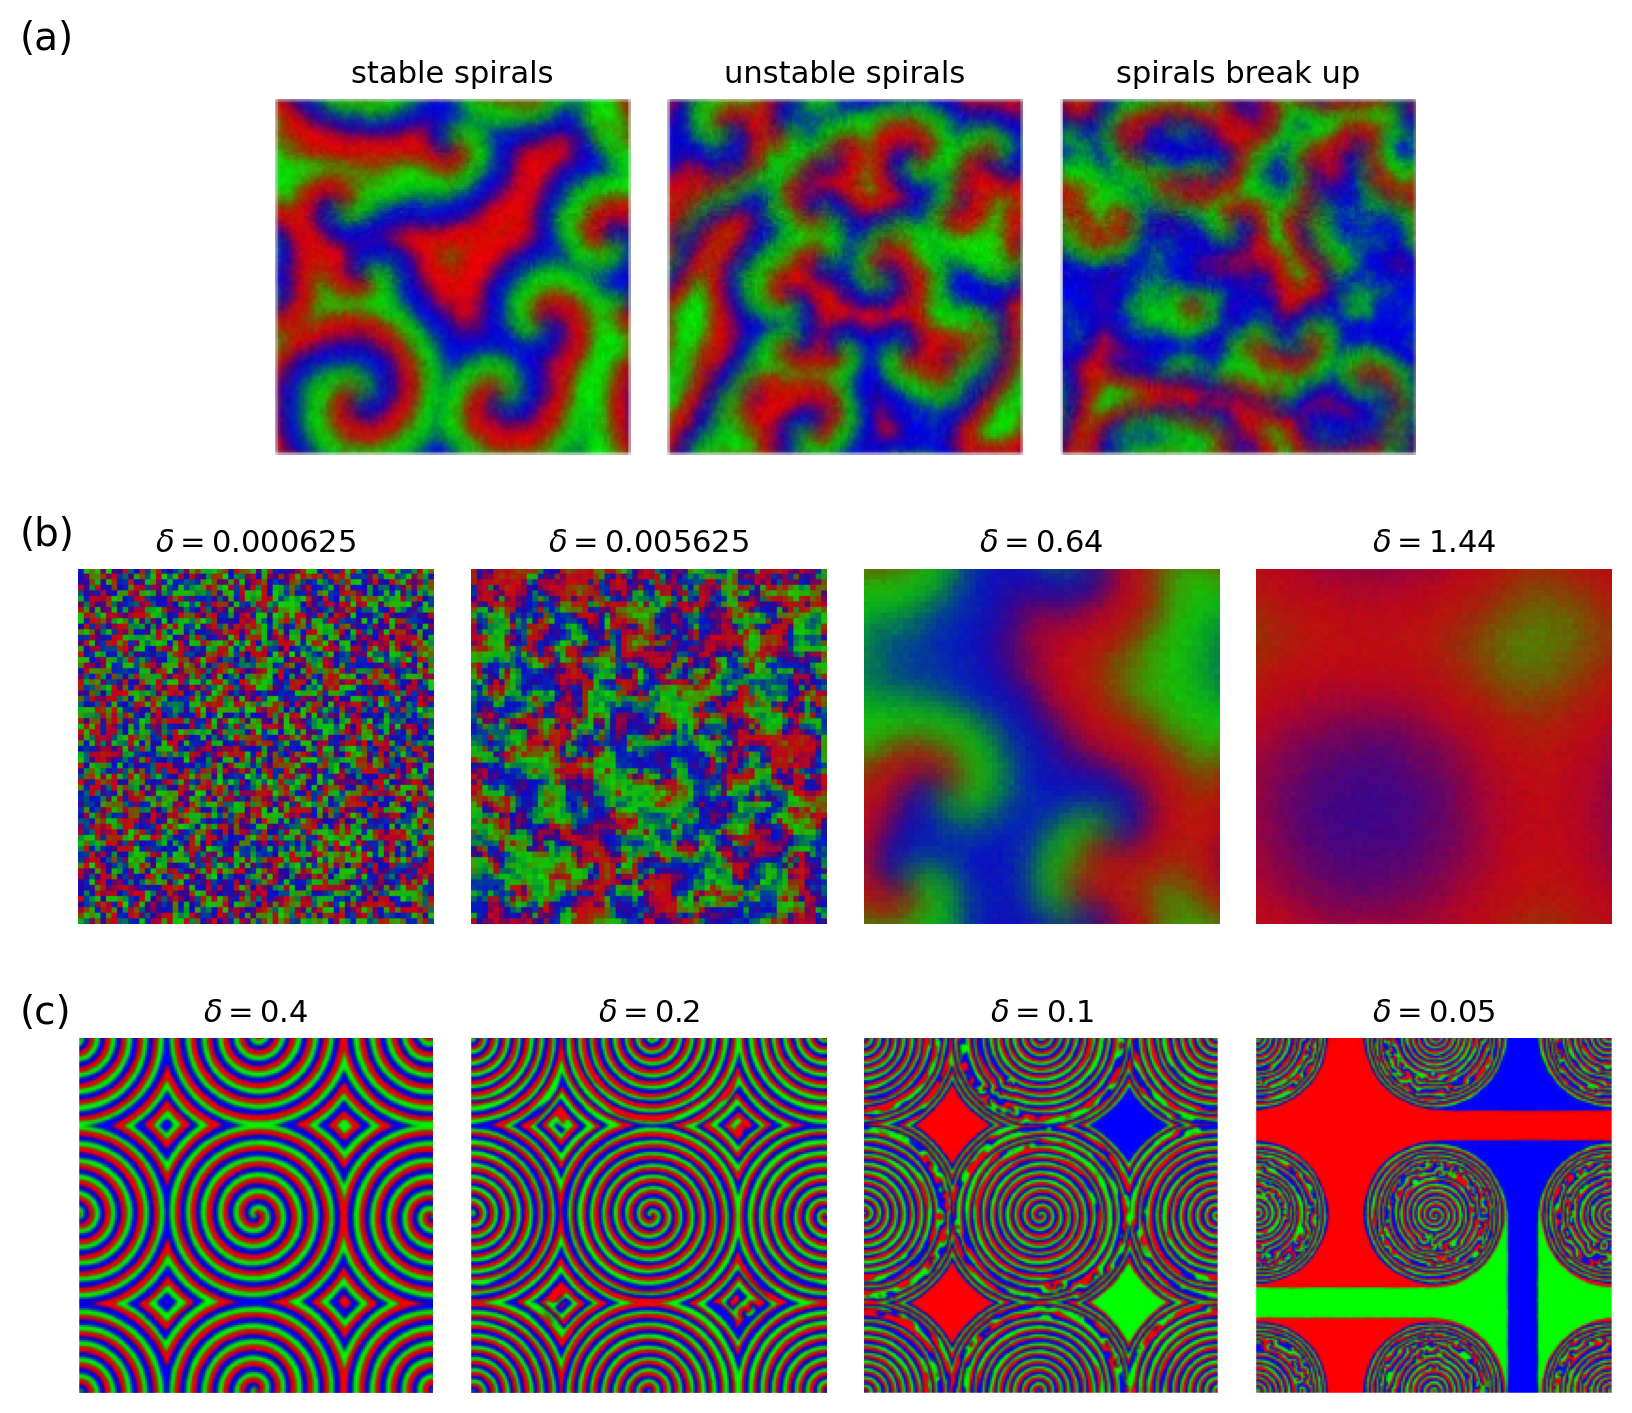
\includegraphics[width=0.9\textwidth]{figures/10_mathematical_ecology/Mobilia2016-spirals.png}
\caption{Spiral waves in stochastic lattice simulations of a spatial rock--paper--scissors model. Each color is one species; $\delta$ is the mobility rate. (a) Depending on parameters, spirals are stable, unstable, or break up. (b) Increasing mobility: no visible pattern, small domains, spirals, and then patterns larger than the system, where one species takes over. (c) Clean spirals at high mobility. Figures~3, 4, and 5 of \hrefc{https://doi.org/10.3390/g7030024}{Mobilia, Rucklidge \& Szczesny, Games (2016)}, licensed under \hrefc{https://creativecommons.org/licenses/by/4.0/}{CC BY 4.0}.}
\label{fig:reich-spirals}
\end{center}
\end{figure}

\clearpage

\subsection*{Early warning signals of tipping points}

\begin{itemize}
\item Many ecosystems can sit in one of alternative stable states
	\begin{itemize}
	\item clear vs.\,turbid lakes,
	\item vegetated vs.\,desert drylands,
	\item coral- vs.\,algae-dominated reefs. 
	\end{itemize}
\item As a slowly changing driver (nutrient loading, grazing, temperature, $\ldots$) crosses a threshold, the system undergoes a catastrophic (most commonly, fold/saddle-node) bifurcation and shifts to the contrasting state. 
\item Such shifts are often hard to reverse (\emph{hysteresis}) and hard to predict.
\end{itemize}

\begin{figure}[h]
\begin{center}
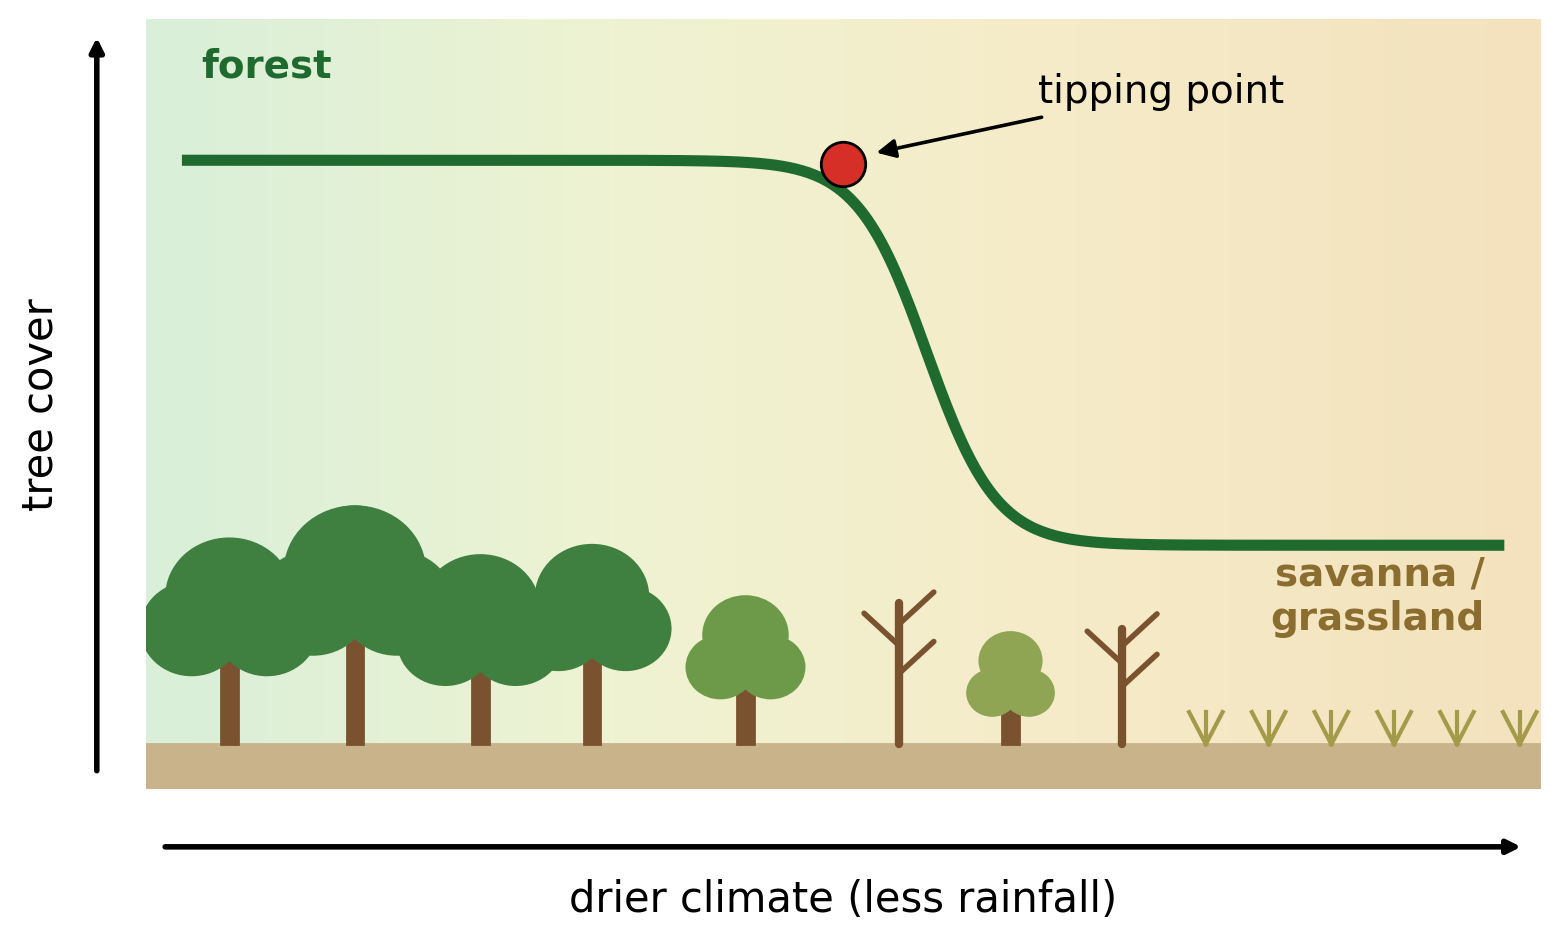
\includegraphics[width=0.7\textwidth]{figures/10_mathematical_ecology/tipping-schematic.png}
\caption{Schematic of a tipping point: as the climate gets drier, tree cover declines slowly at first and then collapses abruptly, turning forest into savanna or grassland.}
\label{fig:tipping-schematic}
\end{center}
\end{figure}

Can we anticipate an approaching tipping point from monitoring data, before it happens by math ($+$ computation)?

\subsubsection*{Critical slowing down}

\begin{itemize}
\item Near a bifurcation, the dominant eigenvalue (the recovery rate $\lambda$ at the equilibrium) approaches zero. The system therefore recovers more and more slowly from small perturbations, a phenomenon called \emph{critical slowing down} (\hrefc{https://doi.org/10.1038/nature08227}{Scheffer et al., Nature (2009)}; \hrefc{https://doi.org/10.1126/science.1225244}{Scheffer et al., Science (2012)}).

\begin{figure}[h]
\begin{center}
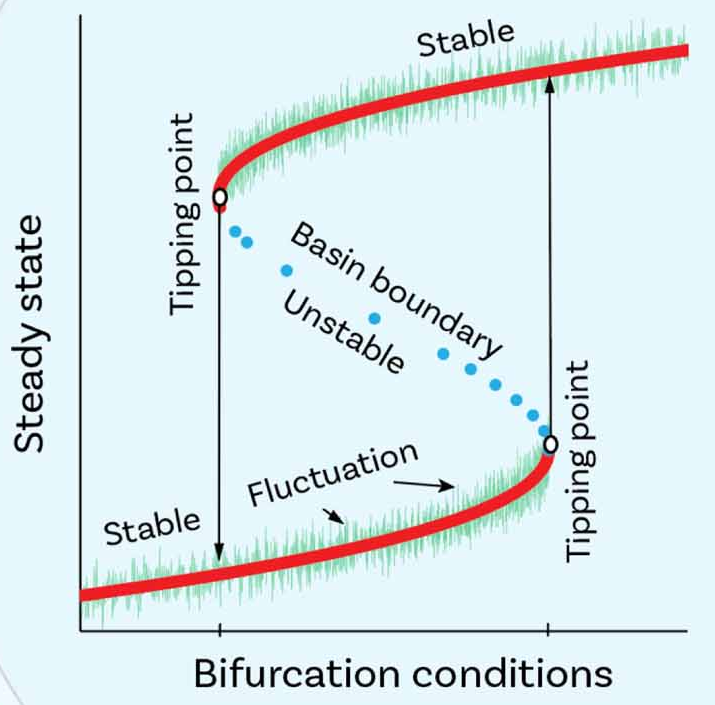
\includegraphics[width=0.34\textwidth]{figures/10_mathematical_ecology/Yi2025ERL-fig1-fold.png}
\hfill
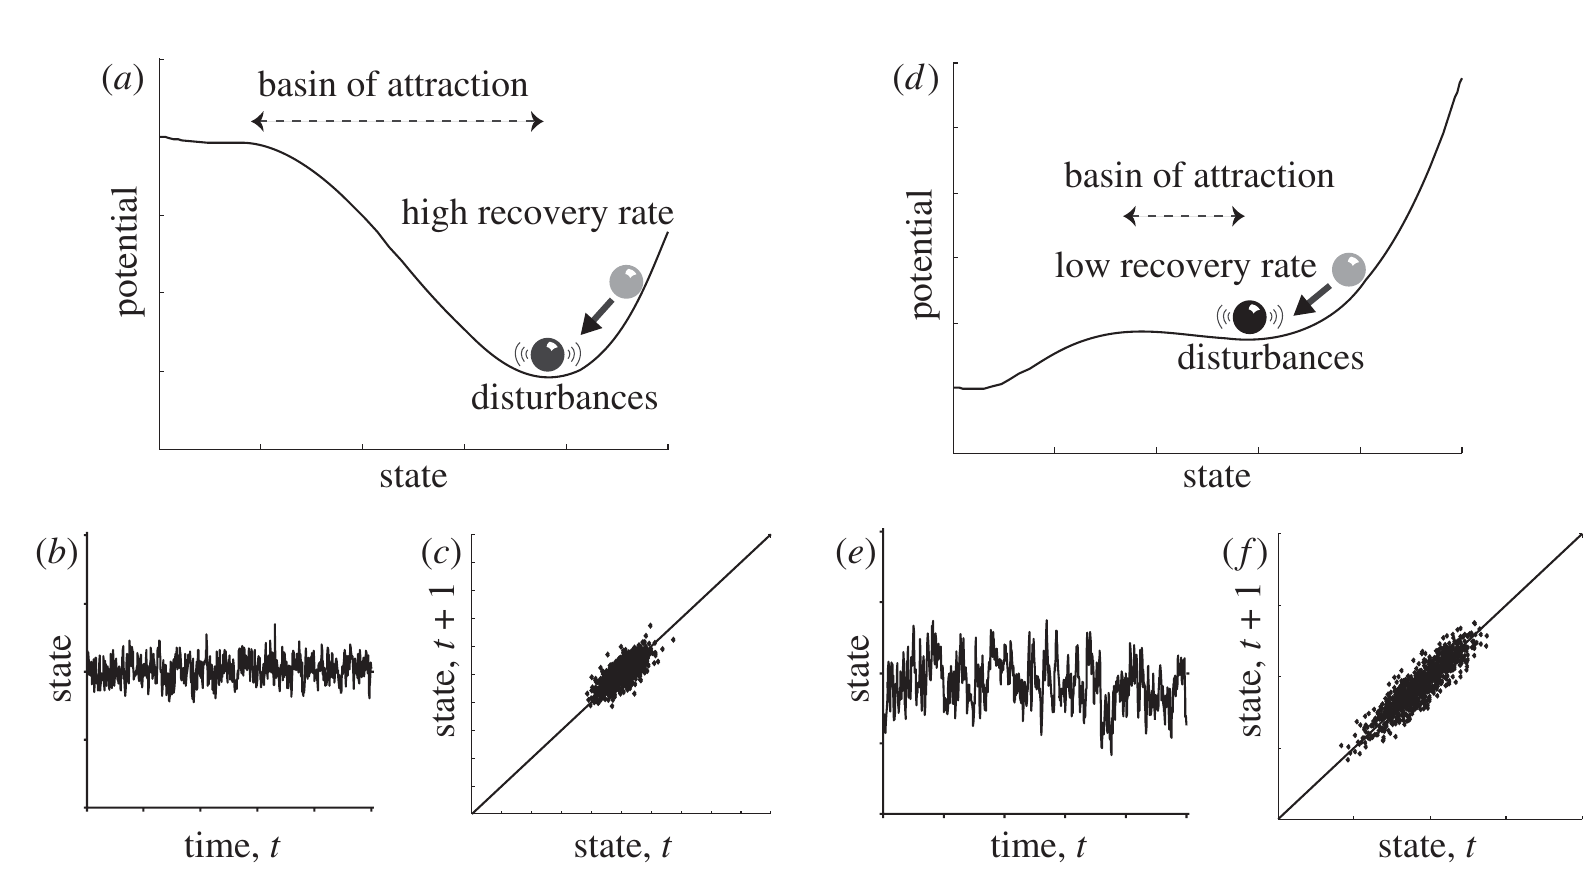
\includegraphics[width=0.62\textwidth]{figures/10_mathematical_ecology/Lenton2012PhilTransA-fig1.png}
\caption{Left: from \hrefc{https://doi.org/10.1088/1748-9326/adb7f3}{Yi et al., Environ. Res. Lett. (2025)}, Fig.~1 (cropped), licensed under \hrefc{https://creativecommons.org/licenses/by/4.0/}{CC BY 4.0}. Right: from \hrefc{https://doi.org/10.1098/rsta.2011.0304}{Lenton et al., Phil. Trans. R. Soc. A (2012)}, Fig.~1, licensed under \hrefc{https://creativecommons.org/licenses/by/3.0/}{CC BY 3.0}.}
\label{fig:critical-slowing-down}
\end{center}
\end{figure}

For example,
\[
\frac{\text{d}x}{\text{d}t} = x\left(1-\frac{x}{K} \right) - c \frac{x^2}{x^2+1} + \text{noise},
\]
where
	\begin{itemize}
	\item $x$: population density
	\item $K$: carrying capacity
	\item $c$: maximum harvest rate
	\end{itemize}	
\item For a monitored time series $x_1, x_2, \ldots, x_L$ with sample mean $\overline{x} = \frac{1}{L}\sum_{\ell=1}^{L} x_{\ell}$,
	\begin{itemize}
	\item variance
	\[ V = \frac{1}{L}\sum_{\ell=1}^{L} (x_{\ell} - \overline{x})^2, \]
	\item lag-1 autocorrelation (the correlation between the series and itself shifted by one time step)
	\[ \rho_1 = \frac{\sum_{\ell=1}^{L-1} (x_{\ell} - \overline{x})(x_{\ell+1} - \overline{x})}{\sum_{\ell=1}^{L} (x_{\ell} - \overline{x})^2}. \]
	\end{itemize}
\item Math shows that, as the tipping point is approached, $\lambda \to 0^-$, and
	\begin{itemize}
	\item $V \propto \frac{1}{\left|\text{Re}(\lambda)\right|} \to \infty$, and
	\item $\rho_1 \to 1$.
	\end{itemize}
Rising variance and rising lag-1 autocorrelation are thus \emph{early warning signals}.
\end{itemize}

\begin{figure}[h]
\begin{center}
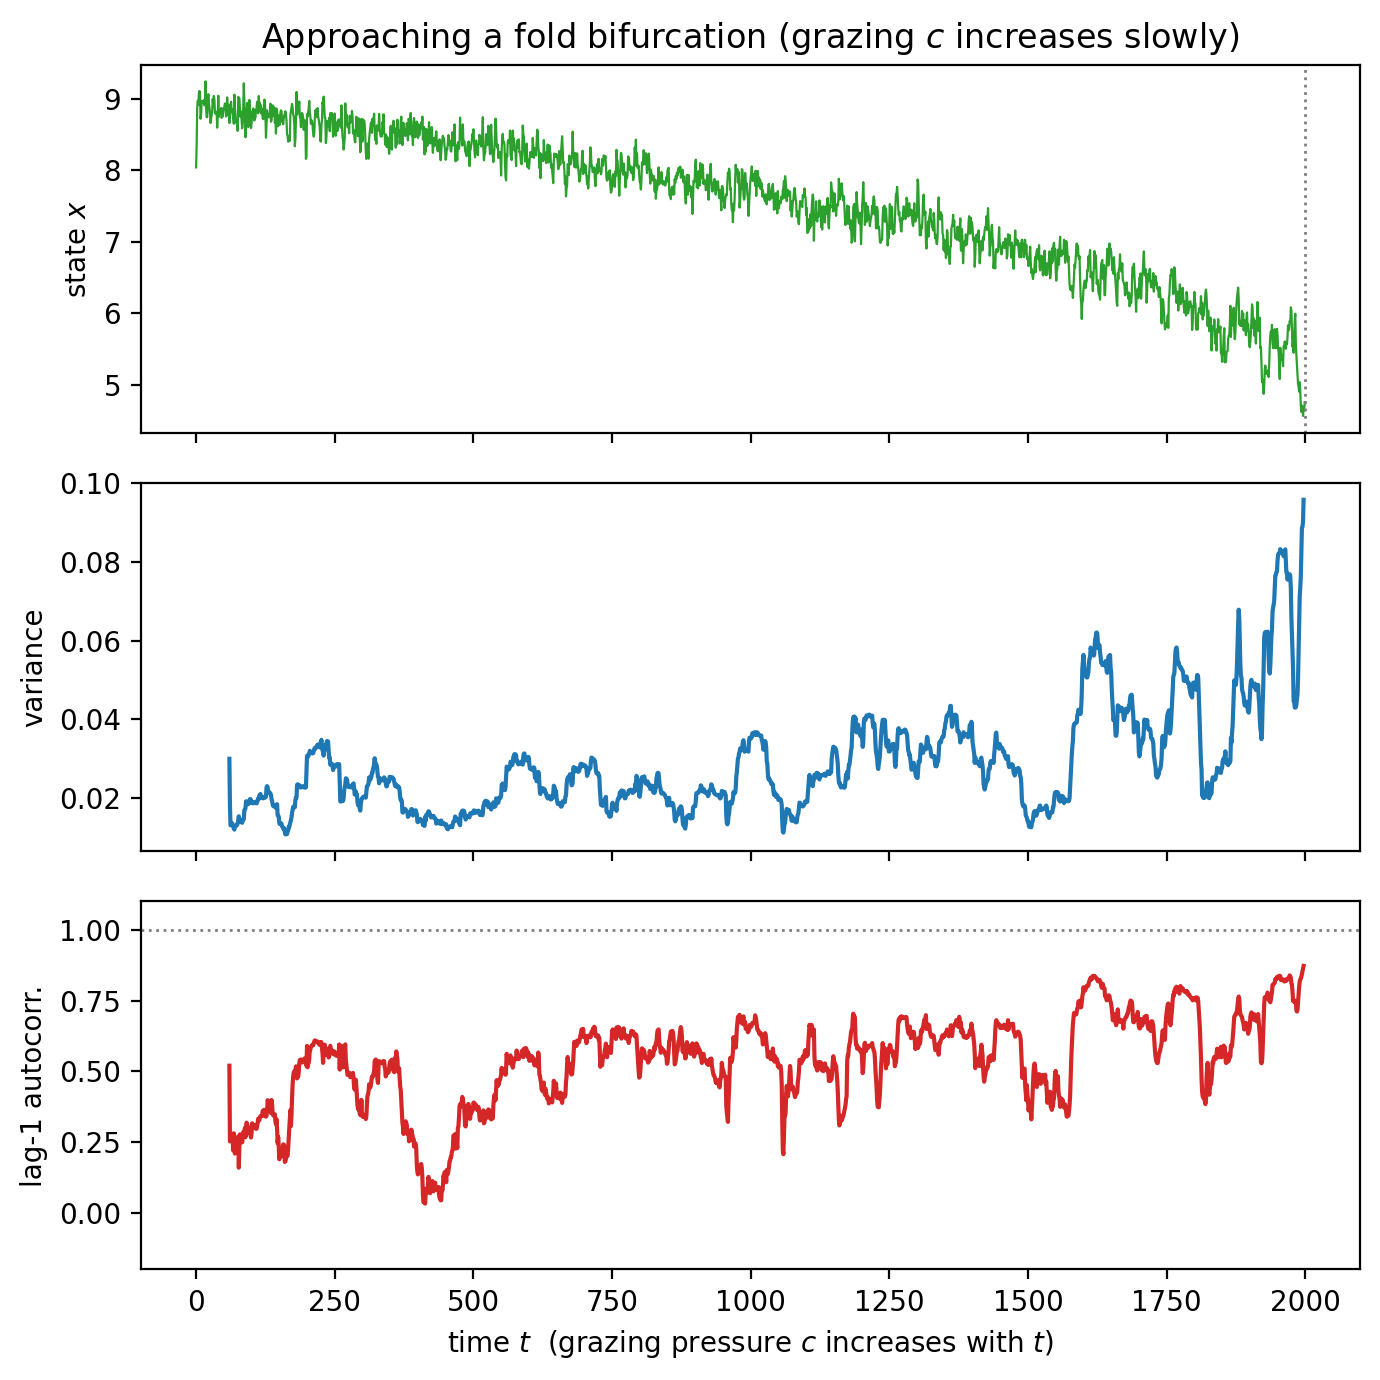
\includegraphics[width=0.65\textwidth]{figures/10_mathematical_ecology/early-warning-signals.png}
\caption{Simulation of the grazing model $\dot{x}=x\left( 1-\frac{x}{K} \right) -c(t) \frac{x^2}{x^2+1}+\text{noise}$ with $c$ increased slowly toward the saddle-node bifurcation. Top: the state $x$ with growing fluctuations before the collapse. Middle and bottom: rolling-window variance and lag-1 autocorrelation both rise as the tipping point is approached.}
\label{fig:ews-sim}
\end{center}
\end{figure}

\clearpage

\subsubsection*{Experimental validation: a whole-lake experiment}

\begin{itemize}
\item \hrefc{https://doi.org/10.1126/science.1203672}{Carpenter et al., Science (2011)} ran a whole-ecosystem test. They gradually added a top predator (largemouth bass) to one lake over three years to drive a food-web regime shift, while monitoring an adjacent reference lake (no manipulation) to control for weather and other shared drivers.
\item In the manipulated lake (but not the reference lake), the early-warning indicators --- variance, lag-1 autocorrelation, skewness, and a shift of the variance spectrum to low frequencies --- rose more than a year \emph{before} the food-web transition completed.
\item Theory vs.\ practice:
	\begin{itemize}
	\item In the idealized bifurcation theory, the variance diverges.
	\item In a real ecosystem, nothing actually diverges to infinity. The indicators merely rise and become detectable.
	\item But, the experiment and what to measure were guided by the theory.
	\end{itemize}
\end{itemize}

\begin{figure}[h]
\begin{center}
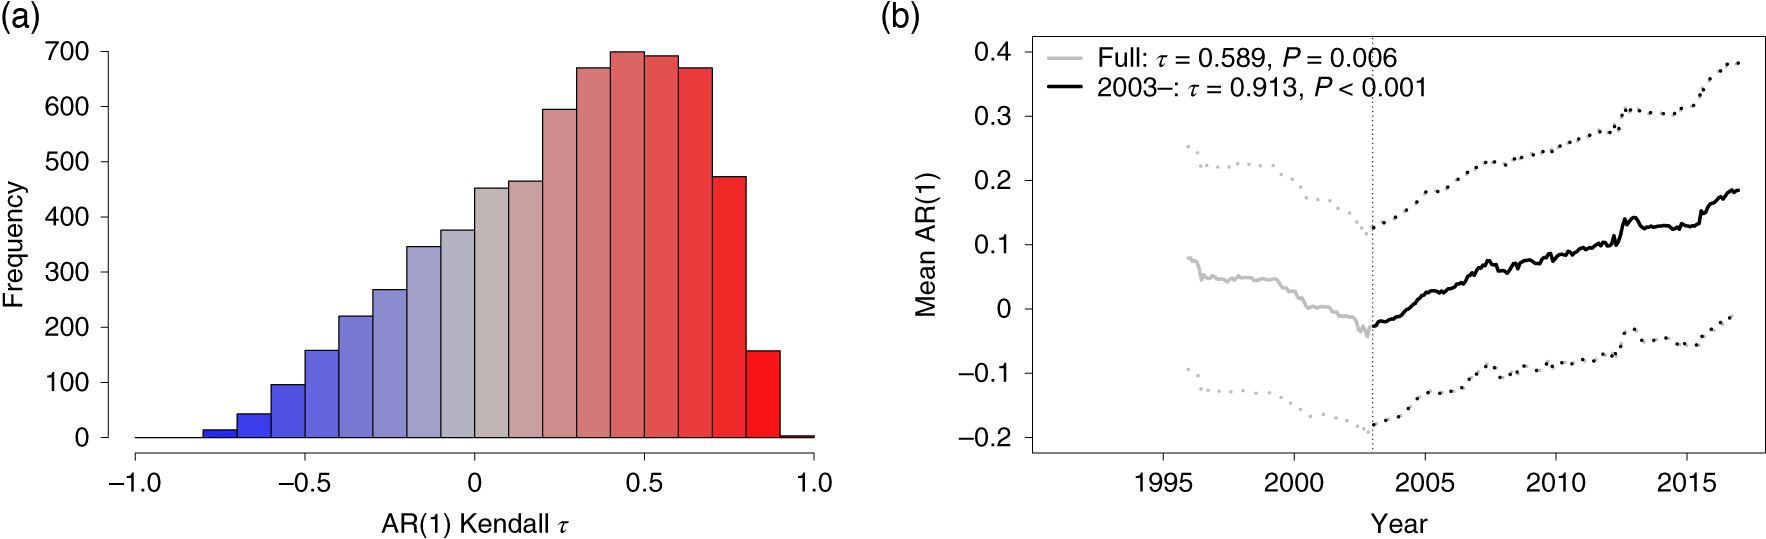
\includegraphics[width=\textwidth]{figures/10_mathematical_ecology/Boulton2022-amazon-ar1.png}
\caption{Another empirical example: loss of resilience of the Amazon rainforest. The data are monthly satellite measurements of vegetation (a proxy for biomass) at each grid cell of the forest. The lag-1 autocorrelation, AR(1), is computed in 5-year sliding windows. (a) Histogram, over grid cells, of the Kendall rank correlation $\tau$ between AR(1) and time from 2003 onwards. A positive $\tau$ suggests critical slowing down. About 76\% of the grid cells have $\tau>0$. (b) AR(1) averaged over grid cells (solid line; dotted lines: $\pm1$ standard deviation). Since 2003, the mean AR(1) has risen almost monotonically ($\tau=0.91$, $P<0.001$). (a) and (b) thus show a positive early warning signal, consistent with the forest approaching a tipping point, although no transition has occurred yet. Adapted from Fig.~2 of \hrefc{https://doi.org/10.1038/s41558-022-01287-8}{Boulton, Lenton \& Boers, Nature Climate Change (2022)}, licensed under \hrefc{https://creativecommons.org/licenses/by/4.0/}{CC BY 4.0}.}
\label{fig:boulton}
\end{center}
\end{figure}

\begin{figure}[h]
\begin{center}
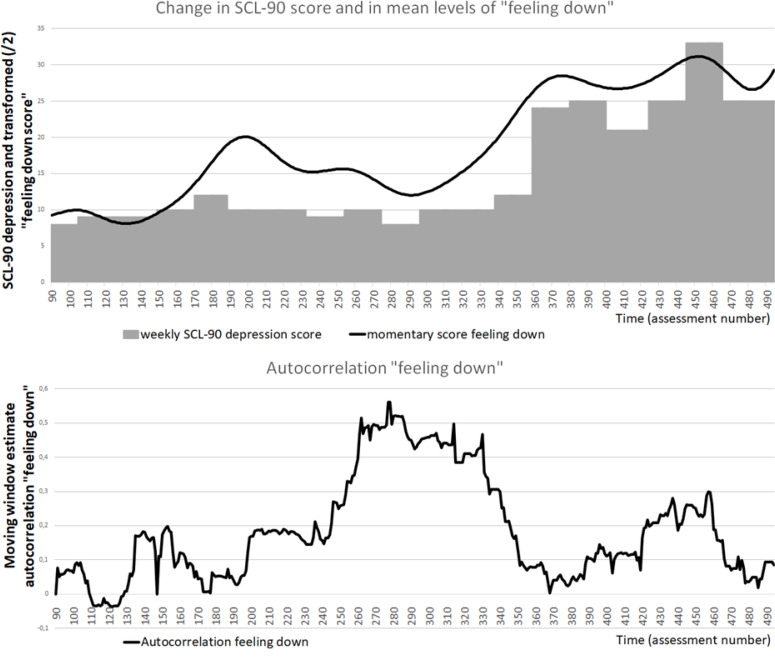
\includegraphics[width=0.78\textwidth]{figures/10_mathematical_ecology/Wichers2020-ews-depression.png}
\caption{Same ideas for depressive symptoms in one individual. Top: weekly depressive symptoms (gray bars) and the smoothed level of momentary ``feeling down'' (black line). A sudden transition to higher symptom levels occurs around assessment 350. Bottom: autocorrelation (which is a major early warning signal based on critical slowing down) of ``feeling down'' estimated in a 30-day moving window. It rises about a month before the transition. Adapted from Fig.~1 of \hrefc{https://doi.org/10.17505/jpor.2020.22042}{Wichers, Smit \& Snippe, J.\ Person-Oriented Res.\ (2020)}, licensed under \hrefc{https://creativecommons.org/licenses/by/4.0/}{CC BY 4.0}.}
\label{fig:Wichers}
\end{center}
\end{figure}

\end{document}
